\documentclass[tikz]{standalone}
\usepackage{pgfplots}
\usepgfplotslibrary{groupplots}
\pgfplotsset{width=13.cm, height=7cm, compat=1.18}
\usepackage{tikz}
\usepackage{amsmath}
\usepackage{amssymb}

\definecolor{darkgray176}{RGB}{176,176,176}
\definecolor{magenta}{RGB}{255,0,255}
\definecolor{mediumblue}{RGB}{0,0,205}
\definecolor{mediumpurple}{RGB}{147,112,219}

\begin{document}
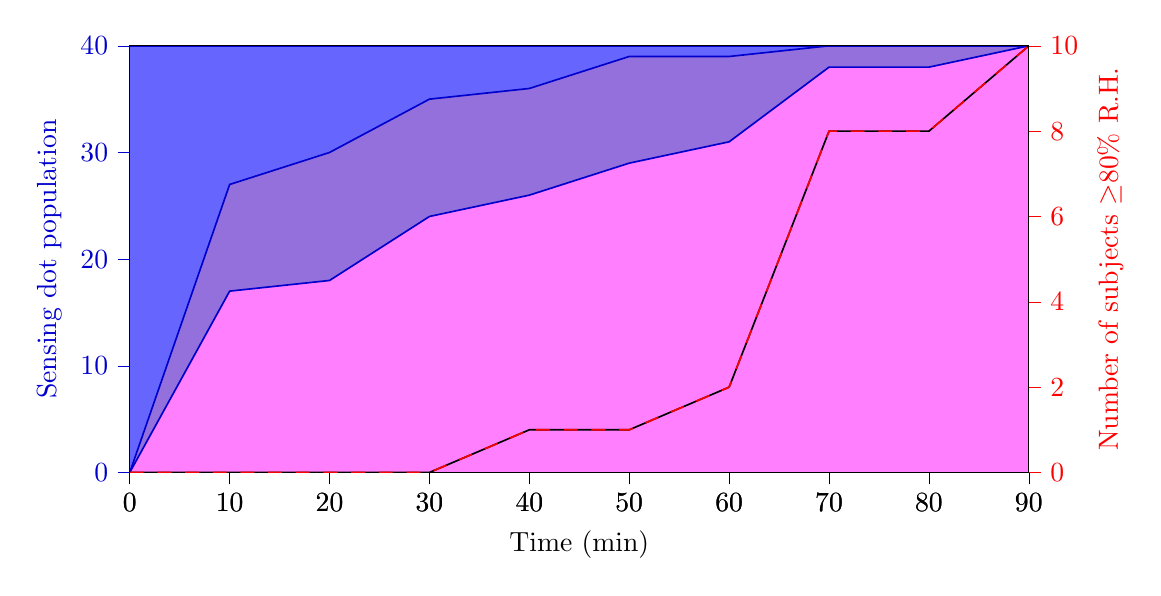
\begin{tikzpicture}
	\begin{axis}[
		tick align=outside,
		tick pos=left,
		% X
		xmin=0, xmax=90,
		xlabel={Time (min)},
		xtick style={color=black},
		% Y
		ymin=0, ymax=40,
		ytick style={mediumblue},
		yticklabel style={color=mediumblue},
		ylabel style = {color=mediumblue},
		ylabel={Sensing dot population},
		]
		\path [fill=blue, opacity=0.6]
		(axis cs:0,0)
		--(axis cs:0,40)
		--(axis cs:10,40)
		--(axis cs:20,40)
		--(axis cs:30,40)
		--(axis cs:40,40)
		--(axis cs:50,40)
		--(axis cs:60,40)
		--(axis cs:70,40)
		--(axis cs:80,40)
		--(axis cs:90,40)
		--(axis cs:90,40)
		--(axis cs:90,40)
		--(axis cs:80,40)
		--(axis cs:70,40)
		--(axis cs:60,39)
		--(axis cs:50,39)
		--(axis cs:40,36)
		--(axis cs:30,35)
		--(axis cs:20,30)
		--(axis cs:10,27)
		--(axis cs:0,0)
		--cycle;
		
		\path [fill=mediumpurple]
		(axis cs:0,0)
		--(axis cs:0,0)
		--(axis cs:10,27)
		--(axis cs:20,30)
		--(axis cs:30,35)
		--(axis cs:40,36)
		--(axis cs:50,39)
		--(axis cs:60,39)
		--(axis cs:70,40)
		--(axis cs:80,40)
		--(axis cs:90,40)
		--(axis cs:90,40)
		--(axis cs:90,40)
		--(axis cs:80,38)
		--(axis cs:70,38)
		--(axis cs:60,31)
		--(axis cs:50,29)
		--(axis cs:40,26)
		--(axis cs:30,24)
		--(axis cs:20,18)
		--(axis cs:10,17)
		--(axis cs:0,0)
		--cycle;
		
		\path [fill=magenta, opacity=0.5]
		(axis cs:0,0)
		--(axis cs:0,0)
		--(axis cs:10,17)
		--(axis cs:20,18)
		--(axis cs:30,24)
		--(axis cs:40,26)
		--(axis cs:50,29)
		--(axis cs:60,31)
		--(axis cs:70,38)
		--(axis cs:80,38)
		--(axis cs:90,40)
		--(axis cs:90,0)
		--(axis cs:90,0)
		--(axis cs:80,0)
		--(axis cs:70,0)
		--(axis cs:60,0)
		--(axis cs:50,0)
		--(axis cs:40,0)
		--(axis cs:30,0)
		--(axis cs:20,0)
		--(axis cs:10,0)
		--(axis cs:0,0)
		--cycle;
		
		\addplot [semithick, mediumblue]
		table {%
			0 40
			10 40
			20 40
			30 40
			40 40
			50 40
			60 40
			70 40
			80 40
			90 40
		};
		\addplot [semithick, mediumblue]
		table {%
			0 0
			10 17
			20 18
			30 24
			40 26
			50 29
			60 31
			70 38
			80 38
			90 40
		};
		\addplot [semithick, mediumblue]
		table {%
			0 0
			10 27
			20 30
			30 35
			40 36
			50 39
			60 39
			70 40
			80 40
			90 40
		};
		\addplot [semithick, mediumblue]
		table {%
			0 0
			10 0
			20 0
			30 0
			40 0
			50 0
			60 0
			70 0
			80 0
			90 0
		};
	\end{axis}
	
	\begin{axis}[
		tick align=outside,
		% X
		xmin=0, xmax=90,
		xtick pos=left,
		xtick style={color=black},
		% Y
		ylabel=\textcolor{red}{Number of subjects $\geq$80\% R.H.},
		ymin=0, ymax=10,
		ytick pos=right,
		ytick style={color=red},
		yticklabel style={anchor=west, color=red}
		]
		\addplot [semithick, black]
		table {%
			0 0
			10 0
			20 0
			30 0
			40 1
			50 1
			60 2
			70 8
			80 8
			90 10
		};
		\addplot [semithick, red, dash pattern=on 5pt off 5pt]
		table {%
			0 0
			10 0
			20 0
			30 0
			40 1
			50 1
			60 2
			70 8
			80 8
			90 10
		};
	\end{axis}
	
\end{tikzpicture}
\end{document}